\documentclass[12pt,titlepage]{article}

\usepackage[utf8]{inputenc}
\usepackage[ngerman]{babel}
\usepackage[latin1]{inputenc}
\usepackage{color}
\usepackage[a4paper,lmargin={4cm},rmargin={2cm},
tmargin={2.5cm},bmargin = {2.5cm}]{geometry}

\usepackage[labelfont={bf, sf},font={small}, labelsep=colon]{caption}
\usepackage{amssymb, amsthm, graphicx, csquotes, floatrow, wrapfig, wasysym, chronology}

\usepackage[backend = biber, style = alphabetic, sorting = nyt]{biblatex}
\DeclareLanguageMapping{ngerman}{ngerman-apa}
\addbibresource{literatur.bib}
\linespread{1.25}
\selectfont
\pagenumbering{arabic}
\DefineBibliographyStrings{ngerman}{%
	andothers = {et\addabbrvspace al\adddot},
	andmore = {et\addabbrvspace al\adddot},
}

%\setcapindent{0.2cm}

\begin{document}
\renewcommand{\figurename}{Abb.}

	
\begin{titlepage} % Format der Uni fehlt noch
		\title{Kolorieren historischer Fotos der
			Stadt Leipzig}
		\date{2022}
		\author{Daniel Grohmann}
		\maketitle
\end{titlepage}

\begin{abstract}
    bla bla dies ist eine Zusammenfassung
\end{abstract}

    \pagebreak
    
\tableofcontents

    \pagebreak
    
\listoffigures
    \pagebreak
    
\section{Einleitung}

\subsection{Motivation}
 (Copy Paste vom Expos\'e, wird noch ge"andert)
 
 
Das F"arben alter Schwarz-Wei\ss-Fotos ist f"ur viele, die sich damit besch"aftigen, ein spa\ss iges
Gimmick, etwas zum Probieren oder wird zur Befriedigung der eigenen Neugier genutzt: Man fragt
sich, wie das Elternhaus, welches "uber Jahrzehnte von Generation zu Generation weitervererbt
wurde, ausgesehen haben kann. Oder - mit diesem verbunden - wie die Ururgro\ss eltern in Farbe
aussahen, um sie oder ihren Kleidungsstil mit dem der lebenden Familienmitglieder zu vergleichen.
Au\ss erdem versuchen professionelle Koloristen, "uberlieferte Kunstwerke und Fotos realistisch zu
modernisieren und ihnen neues Leben einzuhauchen. Jedoch ist gerade die Realit"atsn"ahe beim
Kolorieren historischer Fotos eine - vielleicht die gr"o\ss te - Herausforderung. Es ist nie einhundert
Prozent m"oglich zu sagen, dass diese Person oder dieses bestimmte Geb"aude damals wirklich so
aussah, es sei denn, es existiert ein farbiges Pendant. Deshalb ist der Ansporn der meisten
fachkundigen Koloristen eher die Plausibilit"at. Es wird versucht, die Objekte auf den Fotos so
darzustellen, wie sie wom"oglich ausgesehen haben k"onnten.

Doch mittlerweile sind die Zeiten, in denen man historische Fotos h"ochstaufw"andig manuell F"arben
musste, durch den technologischen Fortschritt und kluge K"opfe wie Jason Antic, Emil Wallner (...)
Geschichte.
Durch die Entwicklung der letzten Jahre im Bereich des Maschinellen Lernens ist der Akt des
F"arbens durch Programme wie DeOldify, OpenCV, Picture Colorizer, AKVIS Coloriage und
Photomyne so benutzernah und leicht zug"anglich wie nie. So ist beispielsweise letzteres sogar als
Applikation f"ur Tablets und Smartphones erh"altlich.

    \pagebreak
\subsection{Ziele der Arbeit}

\subsection{Aufbau der Arbeit}

    \pagebreak
    
\section{Grundlagen}

\subsection{Anf"ange der Fotografie}
Die Camera obscura, welche urspr"unglich nur ein Raum mit einem lichtdurchl"assigen Loch war, beschrieb den ersten Mechanismus, ein vom menschlichen Auge erkanntes Bild (zumindest tempor"ar) zu projizieren. Erste "Uberlieferungen von Anwendungen dieses Mechanismus gibt es laut \textsc{Lef\'evre \cite{lefevre2007inside}} erst im 17. Jahrhundert, wobei vermutet wird, dass dieses Ph"anomen bereits in der Antike entdeckt wurde. Die ersten physischen Exemplare in verschiedenen Formen beinhalteten nur eine einzige konvexe Linse. Die Bilderzeugung erfolgte lediglich mithilfe von extern einstr"omendem Sonnenlicht, welches durch Brechung in der Linse ein reales, invertiertes Abbild auf einer dahinterliegenden Oberfl"ache erzeugte. Dieses konnte daraufhin von K"unstlern in einem umst"andlichen Prozess des Rotierens und Wendens (analog zur Umkehrung eines Negativs mit einer aktuellen Kamera) abgepaust oder abgezeichnet werden.
Neben der gro\ss en Wertsch"atzung f"ur die Welt der Kunst war die Camera obscura in der Astronomie als Observationsmittel, in der Anatomie zum Verstehen des menschlichen Auges und in der Ergr"undung der wissenschaftlichen Optik von wesentlicher Bedeutung. \textsc{\cite{lefevre2007inside, mills1998vermeer}}

Erst im Jahr 1826 gelang es, die fl"uchtigen Bilder in der Dunkelkammer zu fixieren und somit das erste "richtige" \ Foto herzustellen.
Der Franzose Joseph Nic\'ephore Ni\'epce gilt als der Erfinder des ersten Verfahrens, welches dauerhafte Bilder erzeugen konnte, der sogenannten Heliografie. Ihm gelang es, mithilfe von einer d"unnen Asphaltschicht, welche in Lavandel"ol gel"ost und anschlie"send auf einer versilberten Kupfer- oder Zinnplatte angebracht wurde, den Blick aus seinem Arbeitszimmer als Fotografie bei einer Belichtungszeit von ungef"ahr acht Stunden zu entwickeln. Diese erste Art der Momenterfassung gilt als die "alteste erhaltene Fotografie (Abb. \ref{fig:niepce}). Gem"a"s \textsc{Eder \cite{eder1884ausfuhrliches}} war Ni\'epces gr"o"ste Herausforderung nun, seine bahnbrechende Entdeckung anwendungsreif und f"ur eine breitere Masse zug"anglich zu machen. Deshalb schloss er sich 1829 mit dem franz"osischen Maler Louis Daguerre zusammen, jedoch gelang es den beiden w"ahrend Ni\'epces Lebenszeiten nicht, das anfangs sehr materiell aufw"andige Verfahren kommerziell nutzbar zu machen. \textsc{\cite{eder1884ausfuhrliches}}
%\begin{wrapfigure}{0.5\textwidth}
%{\caption{View from the Window at Le Gras, 1826. (\textsc {Harry Ransom Center, The University of Texas at Austin.})}
%\label{fig:niepce}}
%{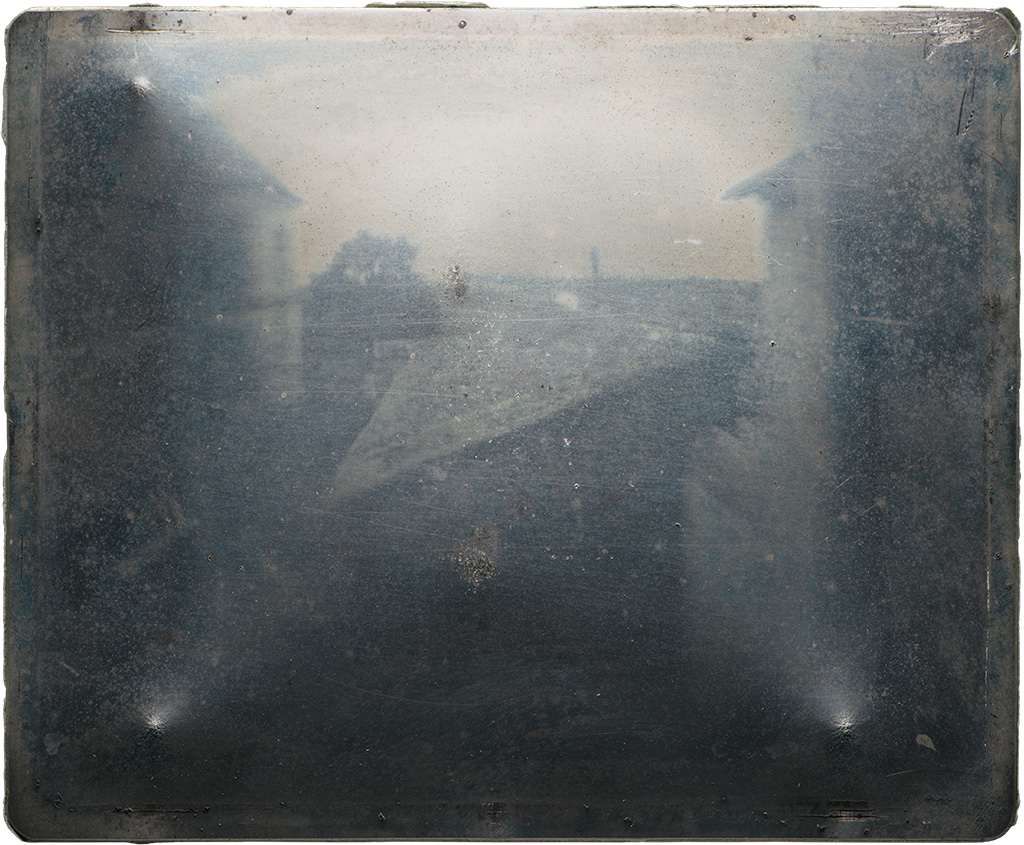
\includegraphics[width=0.4\textwidth]{niepce_heliograph.jpg}}
%\end{wrapfigure}
\begin{figure}[b]

\floatbox[{\capbeside\thisfloatsetup{capbesideposition={right,bottom},capbesidewidth=10cm}}]{figure}[\FBwidth]
{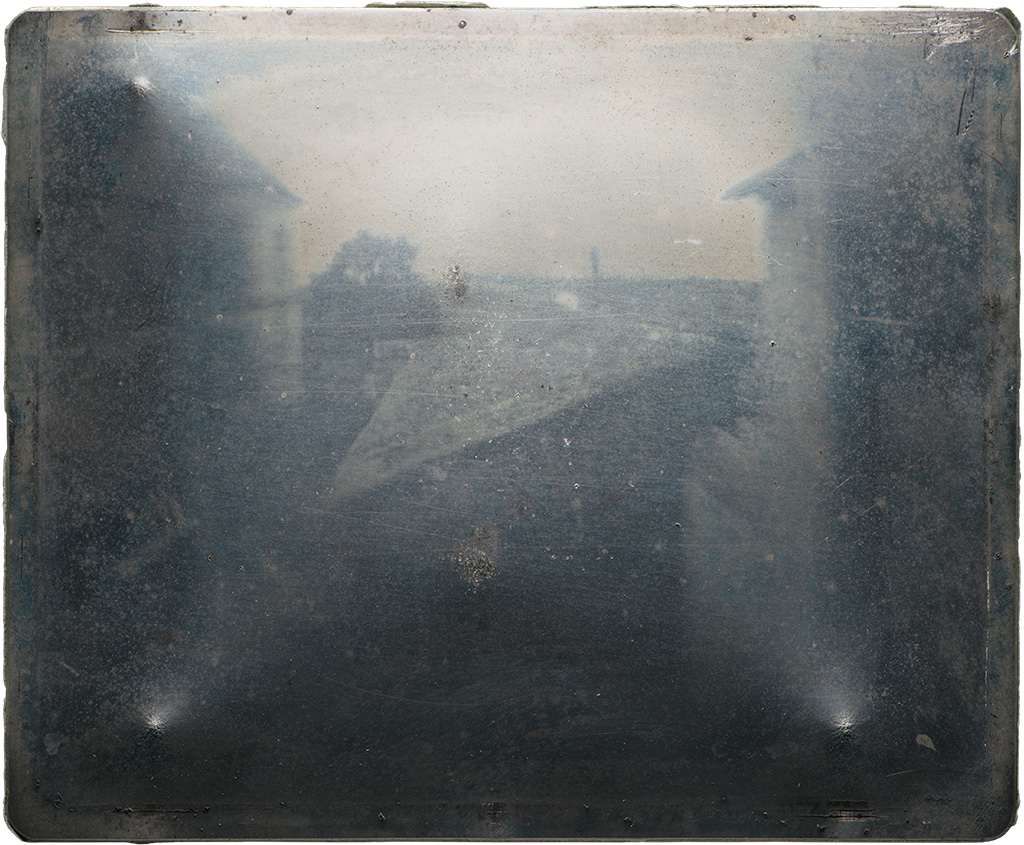
\includegraphics[width=5cm]{niepce_heliograph.jpg}}
{\caption{Blick aus dem Arbeitszimmer in Le Gras, 1826. \textsc {Nicéphore Niépce - Harry Ransom Center's Gernsheim collection, The University of Texas at Austin}}\label{fig:niepce}}

\end{figure}

Erst 1839 gelang es Daguerre, monochrome (schwarz-weiße) Fotos reproduktiv anfertigen zu können. Aufbauend auf den Grundlagen Niépces entdeckte er, dass das Silberiodid allein, was beim Behandeln der versilberten Kupferplatten mit Ioddampf entsteht, durch seine Lichtempfindlichkeit reicht, um Bilder herzustellen. Eine Alternative stellte Quecksilberdampf dar und sorgte für ein ähnliches Ergebnis. Für seine sogenannte Daguerreotypie verwendete er eine verbesserte und kleinere Version der Camera obscura (oder Lochkamera) als Fotoapparat. \textsc{\cite{barger2000daguerreotype}}

Die Daguerrotypie wurde durch darauf aufbauende Methoden wie die Kalotypie, Ambrotypie und Tintypie, welche erste Versuche der Farbfotografie repr"asentierten, erg"anzt und verfeinert \textsc{\cite{lavedrine2009photographs}}. Jedoch blieb die Mehrheit der fotografischen Aufnahmen bis zur Mitte des 20. Jahrhunderts monochrom \textsc{\cite{hacking2012foto}}. 

% evtl noch mehr eingehen auf die Art und Weise der Fotografie Daguerres, Kalo- Ambro- und Tintypie eingehen
\vspace{2cm}
\begin{chronology}[10]{1810}{1905}{\textwidth}
\event{1825}{\small{Erstes Foto (Niépce)}}
\event{1839}{Daguerreotypie}
\event{1861}{Erstes Farbfoto Maxwell}
\event{1888}{Kodak 1}
\event{1900}{Kamera für Massenmarkt}
%\event{1948}{Polaroid Sofortbildkamera}
%\event[1826]{1986}{\small{two}}
%\event{\decimaldate{25}{12}{2001}}{\huge{three}}
\end{chronology} \\

\begin{center}
    (WorkInProgress)
\end{center}
    \pagebreak
    
\subsection{Handkolorierung}

Im Allgemeinen wird das Kolorieren als das F"arben monochromer (schwarz-wei\ss er) Bilder, seien sie bewegt oder unbewegt, definiert \textsc{\cite{luan2007natural}}. Im Englischen wird der Begriff "colorization" \ auch vom Begriff "coloring" \ (oft mit "hand coloring"\ spezifiert) unterschieden. Ersterer beschreibt meist dabei den digitalen Vorgang, letzterer ist älter und an den händischen Prozess angelehnt. In der deutschen Sprache wird diese Differenzierung nicht vorgenommen. Neben der mittelalterlichen Buchmalerei, die den Ursprung der h"andischen Illustrationsf"arbung darstellt, soll in dieser Arbeit aber vor allem auf das F"arben von Fotos eingegangen werden.
% evtl. zur Def noch ne Quelle

Die Handkolorierung von Fotos, wie wir sie heute kennen, wurde direkt nach der Entwicklung erster Daguerrotypien mit verschiedenen Ans"atzen in Angriff genommen und ist somit erstmals auf diese Zeit zur"uckzuf"uhren. Für eine Zusatzgebühr konnte man beim Künstler verlangen, dass das schwarz-weiße Foto nachkoloriert wird. Der Beauftragte notierte sich die Farbe der Kleidung, Augen und Haare des abgebildeten Kunden, falls es sich um ein Portrait handelte \textsc{\cite{hannavy2013encyclopedia}}. Dieses Angebot der nachträglichen Einfärbung war notwendig, da laut Henisch et al. \textsc{\cite{henisch1996painted}} bei Weitem nicht alle Menschen von der "neuen Magie" \ der ersten monochromen Fotos überzeugt waren. Sie vermissten die Farbenfrohheit der Gem"alde, die in ihrem Zuhause hingen, und trachteten danach, ein Gegenmittel zur Monotonie der Abbildungen zu finden. Diese Bestrebungen nach mehr Realismus wurden zu Beginn mit einem Gemisch aus verschiedenen Pigmenten und Gummi Arabicum als Bindemittel erreicht. Unter Hitzeeinfluss wurden die Farbstoffe anschlie\ss end auf den Daguerrotypien fixiert. Johann Baptist Isenring war 1839 der erste K"unstler, der diese Technik nutzte. \textsc{\cite{ferguson2008living, henisch1996painted}} 

Seit der Mitte des 19. Jahrhunderts ist mit den Methoden des fr"uhen Kolorierens stetig weiterexperimentiert wurden, jedoch ohne nennenswerte Fortschritte zu erreichen. Erst einige Jahre sp"ater, mit der Erfindung der Solarkamera und damit einhergehend das Vorhandensein einer ausreichend starken Lichtquelle w"ahrend des Vorgangs, konnten Fotos vergr"o\ss ert auf Papier oder Leinw"anden dargestellt werden \textsc{\cite{towler1873silver}}. So konnten beispielsweise Portraits f"ur das Bearbeiten leichter zug"anglich gemacht und in Lebensgr"o\ss e abgebildet werden. Das durch diese und weitere Errungenschaften vereinfachte Handkolorieren war bis zur Mitte des 20. Jahrhunderts und zur Erfindung des Kodachrome Farbfilms die beliebteste Methode, um gef"arbte Fotografien herzustellen. 
% koennte hier auch noch deeper gehen, moechte aber mich nicht zu lange bei der Geschichte aufhalten
Trotz der Existenz der seitdem deutlich unkomplizierteren Methode und deren Nachfolgern, war das h"andische Kolorieren von Fotos in den folgenden Jahren immer noch von gro\ss er Bedeutung und erlebte in den 1970ern eine Art Wiedergeburt, weil viele Menschen sich nach dem Antiken und Alten sehnten. Bis heute ist die Handkolorierung eine beliebte T"atigkeit, sei es wegen visueller "Asthetik oder der Best"andigkeit der beim Vorgang verarbeiteten Farbpigmente. \textsc{\cite{ivankovich2005early}}
% Diese Quelle bei Bedarf aktualisieren  :)

% Bild Handkolorierung

% erstmal gestrichen wegen verlorener Quelle:
%Doch so einfach wie die Definition ist der Vorgang des F"arbens selbst in keinster Weise. Dabei ist vor allem der zeitliche Aufwand beim professionellen, h"andischen Prozess bis vor ein paar
%Jahren enorm gewesen. F"ur die Recherche von Hintergr"unden und Abstammung der zu kolorierten
%Person und f"ur die Bearbeitungszeit selbst musste man in der Regel bis zu einem Monat einplanen.
%Dies war oft beim farblichen Erneuern eines einzigen Gesichtes der Fall, da zum Beispiel f"ur den
%Hautton allein bis zu zwanzig pinken Farbschichten gebraucht wurden. Hinzu kommt der k"orperliche
%Aspekt und somit, die ausdauernde Konzentration und Fingerfertigkeit zu beweisen.

\subsection{Digitales Kolorieren}

\textsc{Ferguson \cite{ferguson2008living}} behauptet, dass die gewaltigsten H"urden, die es zu bezwingen galt, neben den materiellen Kosten vor allem der k"orperliche und zeitliche Aufwand, monochromen Aufnahmen mit Farben einen neuen Glanz zu verleihen, waren. Das Foto musste erst mit den vorhandenen Praktiken geschossen, entwickelt und gedruckt werden, bevor das Ergebnis von einem - meist demselben - K"unstler in einem oft langwierigen Prozess handgef"arbt werden konnte. Die nachgefragtesten Fotografen und Koloristen besaßen deshalb eine traditionelle künstlerische Ausbildung. Kolorierte Fotos waren deutlich erschwinglicher als echte Gemälde und erwiesen sich in der Öffentlichkeit schnell als lukrativ. \textsc{\cite{ferguson2008living, hoppe2010spectroscopic}}
%Wenn man nicht das Know-How und die Fingerfertigkeit besaß, sie selbst herzustellen, fehlte es häufig an den finanziellen Mitteln, jemanden zu beauftragen. 

Heutzutage ist das Kolorieren haupts"achlich ein rechnergest\"utzter Prozess, wobei der Aufwand des F"arbens praktisch komplett von Programmen und deren Algorithmen "ubernommen wird. Moderne Technologien und der Fortschritt im Bereich der k"unstlichen Intelligenz haben diesen revolutioniert und deutlich vereinfacht. Trotz alledem ist es noch lange kein trivialer Vorgang. Besonders wenn man ausgezeichnete Resultate erwartet, sind eine gewisse Expertise und Erfahrung, gerade wenn es um Fotorestauration geht, fundamental.



%Wilson Markle erkl"arte 1970 das Kolorieren neu als rechnergest\"utzten Prozess, den er erfand, um Farben zu schwarz-wei\ss en Filmen oder Fernsehprogrammen hinzuzuf"ugen. Der erweiterte Schwierigkeitsgrad bei bewegten Bildern


  

    \pagebreak
\section{Verwandte Arbeiten}
    \pagebreak

\section{Neuronale Netze GAN's: Fokus auf DeOldify}
\subsection{Deep Learning Techniken des Kolorierens}

    \pagebreak

\subsection{DeOldify}
    \pagebreak

\section{Implementierung}

    \pagebreak

\section{Evaluation (Vergleich Projekte)}
    \pagebreak

\section{Fazit und Ausblick}

% Beruf Kolorist und Filmfaerbung erwaehnen
    \pagebreak

\section{Selbstst"andigkeitserkl"arung}
    \pagebreak

\section{Literaturverzeichnis}
 \printbibliography
    \pagebreak
    
\section{Anhang}



\end{document}
